\documentclass{beamer}
%\usepackage{xspace}
\usepackage{amsmath,amssymb}
\usepackage{graphicx}
%\usepackage{svg}
%\usepackage{pgfpages}
%\pgfpagesuselayout{4 on 1}[a4paper,border shrink=5mm,landscape]
%\usepackage{psfrag}
%\usepackage[usenames,dvipsnames]{xcolor}
\usepackage{braket}
\usepackage{qcircuit}
%\usepackage{algorithmicx}
\usepackage{algpseudocode}
\usepackage{tikz}
\usepackage{tikz-3dplot}
\usetikzlibrary{circuits.logic.US}
\usetikzlibrary{graphs}
\usetikzlibrary{datavisualization}
\usetikzlibrary{datavisualization.formats.functions}
\usepackage{pgfplotstable}
\usepgfplotslibrary{patchplots}

\setbeamercovered{transparent}

\usetheme{Pittsburgh}
%\usetheme{default}

\setbeamertemplate{sidebar right}{}
\setbeamertemplate{footline}[frame number]
%\usefonttheme{professionalfonts}

%\usepackage{sansmathaccent}
%\usepackage{bm}

%\usepackage{unicode-math}
%%\setmainfont[SlantedFont={Latin Modern Roman Slanted},SlantedFeatures={Color=000000},
%%  SmallCapsFont={TeX Gyre Termes},SmallCapsFeatures={Letters=SmallCaps}]{XITS}
%\setmathfont[math-style=ISO,sans-style=upright]{XITS Math}
%\setmathfont[range={\mathcal,\mathbfcal}]{Latin Modern Math}

\usepackage{sfmath}

%\mathversion{sans}

\newcommand{\Tr}{\mathsf{Tr}}

\definecolor{redorange}{rgb}{1.0, .25, .25}
\definecolor{citation}{rgb}{.1, 0.8, .35}
\newcommand\emm[1]{\textcolor{redorange}{{#1}}}
\newcommand\numc[1]{\textcolor{citation}{{\bf #1}}}

%\newcommand\bm[1]{{\mbox{\boldmath $#1$}}}
\newcommand\bm[1]{{\mathbf{#1}}}
%\newcommand\bm[1]{{\bf #1}}
%\newcommand\bm[1]{\ensuremath{\boldsymbol{#1}}}
%\newcommand\bm[1]{{\textbf{\it #1}}}

\title{Grover's algorithm}
\author{Ryuhei Mori}
%\institute{$\vcenter{\hbox{\includegraphics[width=30pt]{ELC_logo}}}$ Postdoctoral Fellow of ELC\\ $\vcenter{\hbox{\includegraphics[width=20pt]{titech_logo}}}$ Tokyo Institute of Technology}
\institute{Tokyo Institute of Technology}
%\date{21, Feb, 2019}



\begin{document}
\begin{frame}[plain]
\maketitle
\end{frame}


\begin{frame}{Searching problem}
Searching problem:
\begin{equation*}
f: \{1,2,\dotsc,N\}\to\{0,1\}
\end{equation*}
Find $x\in\{1,2,\dotsc,N\}$ satisfying $f(x) = 1$.

\vspace{3em}
\centering
\Large
How many times, do we have to evaluate $f(x)$ ?

\vspace{2em}
\large
Obviously, $O(N)$.
%
%\vspace{2em}
%Grover's algorithm can do this with $\emm{O(\sqrt{N})}$ evaluations.
\end{frame}

\begin{frame}{Quantum searching problem}
Unitary oracle
\begin{equation*}
U_f \ket{x}\ket{y} = \ket{x}\ket{y\oplus f(x)}.
\end{equation*}
Find $x\in\{1,2,\dotsc,N\}$ satisfying $f(x) = 1$.

\vspace{3em}
\centering
\Large
How many times, do we have to evaluate $U_f$ ?

\vspace{2em}
\large
$\emm{O(\sqrt{N})}$ by Grover's algorithm.
\end{frame}

\begin{frame}{Unitary matrix for Grover's algorithm}
Another unitary
\begin{equation*}
V_f \ket{x} = (-1)^{f(x)}\ket{x}.
\end{equation*}

\vspace{2em}
\[
\Qcircuit @C=2em @R=1em {
\lstick{\ket{x_1}}   & \multigate{3}{U_f}&  \qw\\
\lstick{\ket{x_2}}   & \ghost{U_f} & \qw\\
\lstick{\ket{x_3}}   & \ghost{U_f} & \qw\\
\lstick{\ket{-}}     & \ghost{U_f} & \qw
}
\qquad
=
\qquad
\qquad
\Qcircuit @C=2em @R=1em {
\lstick{\ket{x_1}}   & \multigate{2}{V_f}&  \qw\\
\lstick{\ket{x_2}}   & \ghost{V_f} & \qw\\
\lstick{\ket{x_3}}   & \ghost{V_f} & \qw\\
}
\]


\vspace{2em}
\begin{align*}
\ket{x}\ket{-}\longmapsto U_f\ket{x}\ket{-} = (-1)^{f(x)}\ket{x}\ket{-}.
\end{align*}
\end{frame}

\begin{frame}{Grover's algorithm}
\begin{align*}
\ket{\psi} := \frac1{\sqrt{N}} \sum_{x=1}^N \ket{x}
\end{align*}
\begin{align*}
V_f  &= I - 2 \sum_{x: f(x) = 1}\ket{x}\bra{x}\\
W    &:= I - 2 \ket{\psi}\bra{\psi}.
\end{align*}
Then, $G:=WV_f$ is called the Grover's operator.

\vspace{2em}
The Grover's algorithm just measures \emm{$G^k\ket{\psi}$} by the computational basis for some \emm{appropriately chosen} $k$.
\end{frame}



\begin{frame}{The two dimensional subspace}
\begin{align*}
\ket{s} &:= \frac1{\sqrt{M}}\sum_{x: f(x) = 1} \ket{x}\\
\ket{f} &:= \frac1{\sqrt{N-M}}\sum_{x: f(x) = 0} \ket{x}.
\end{align*}
Then,
\begin{align*}
\ket{\psi} = \frac1{\sqrt{N}} \sum_{x=1}^N \ket{x}
&= \sqrt{\frac{M}{N}} \ket{s} + \sqrt{\frac{N-M}{N}} \ket{f}\\
&= \sin\theta\ket{s} + \cos\theta\ket{f}
\end{align*}
where $\theta=\arcsin\sqrt{\frac{M}{N}}$.
\end{frame}

\begin{frame}{Analysis of Grover's algorithm}
\centering
\only<1>{
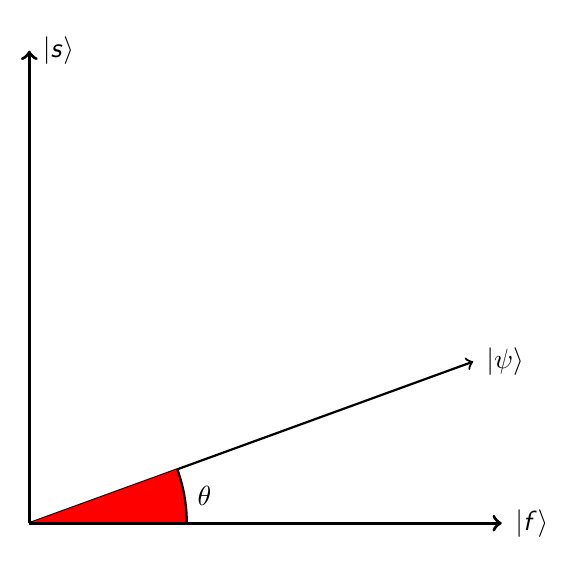
\begin{tikzpicture}
\draw[very thick,->] (0,0) -- (6,0) node[right=1pt] {$\ket{f}$};
\draw[very thick,->] (0,0) -- (0,6) node[right=1pt] {$\ket{s}$};
\draw[thick,->] (0:0) -- (20:6) node[right=1pt] {$\ket{\psi}$};
\filldraw[thick,fill=red] (0,0) -- (2,0) arc[start angle=0, end angle=20, radius=2] node[pos=0.5,right=1pt] {$\theta$};
\end{tikzpicture}
}
\only<2>{
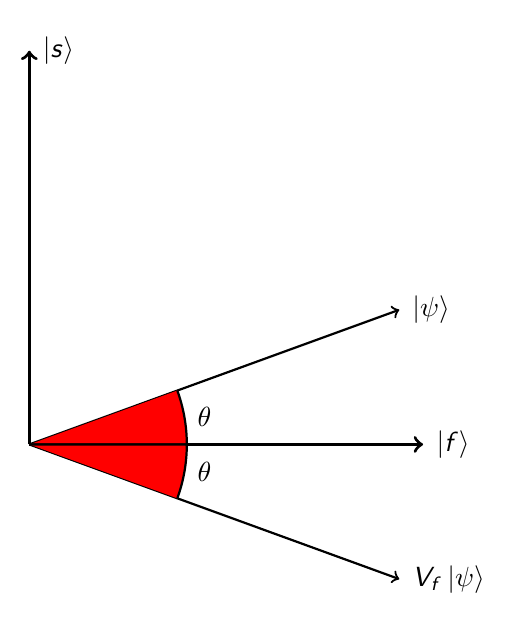
\begin{tikzpicture}
\draw[very thick,->] (0,0) -- (5,0) node[right=1pt] {$\ket{f}$};
\draw[very thick,->] (0,0) -- (0,5) node[right=1pt] {$\ket{s}$};
\draw[thick,->] (0:0) -- (20:5) node[right=1pt] {$\ket{\psi}$};
\filldraw[thick,fill=red] (0,0) -- (2,0) arc[start angle=0, end angle=20, radius=2] node[pos=0.5,right=1pt] {$\theta$};
\draw[thick,->] (0:0) -- (-20:5) node[right=1pt] {$V_f\ket{\psi}$};
\filldraw[thick,fill=red] (0,0) -- (2,0) arc[start angle=0, end angle=-20, radius=2] node[pos=0.5,right=1pt] {$\theta$};
\end{tikzpicture}
}
\only<3>{
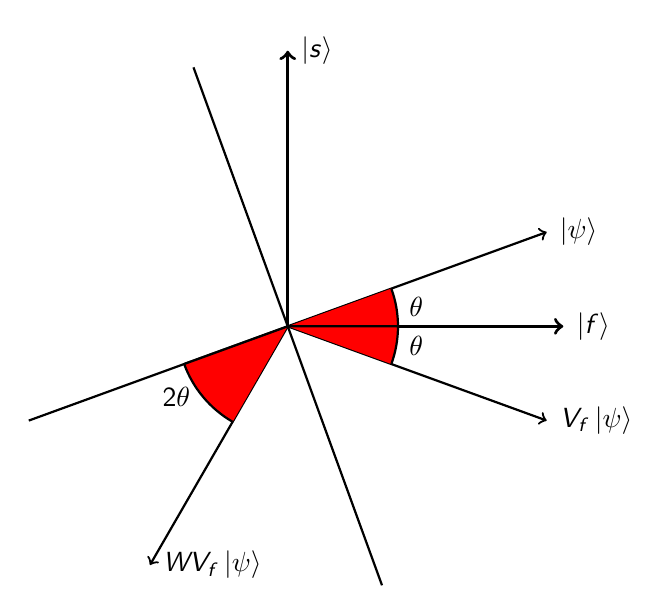
\begin{tikzpicture}[scale=0.7]
\draw[very thick,->] (0,0) -- (5,0) node[right=1pt] {$\ket{f}$};
\draw[very thick,->] (0,0) -- (0,5) node[right=1pt] {$\ket{s}$};
\draw[thick,->] (0:0) -- (20:5) node[right=1pt] {$\ket{\psi}$};
\filldraw[thick,fill=red] (0,0) -- (2,0) arc[start angle=0, end angle=20, radius=2] node[pos=0.5,right=1pt] {$\theta$};
\draw[thick,->] (0:0) -- (-20:5) node[right=1pt] {$V_f\ket{\psi}$};
\filldraw[thick,fill=red] (0,0) -- (2,0) arc[start angle=0, end angle=-20, radius=2] node[pos=0.5,right=1pt] {$\theta$};
\draw[thick] (0:0) -- (110:5);
\draw[thick] (0:0) -- (-70:5);
\draw[thick] (0:0) -- (200:5);
\draw[thick,->] (0:0) -- (240:5) node[right=1pt] {$WV_f\ket{\psi}$};
\filldraw[thick,fill=red] (0,0) -- (200:2) arc[start angle=200, end angle=240, radius=2] node[pos=0.5,left=1pt] {$2\theta$};
\end{tikzpicture}
}
\only<4>{
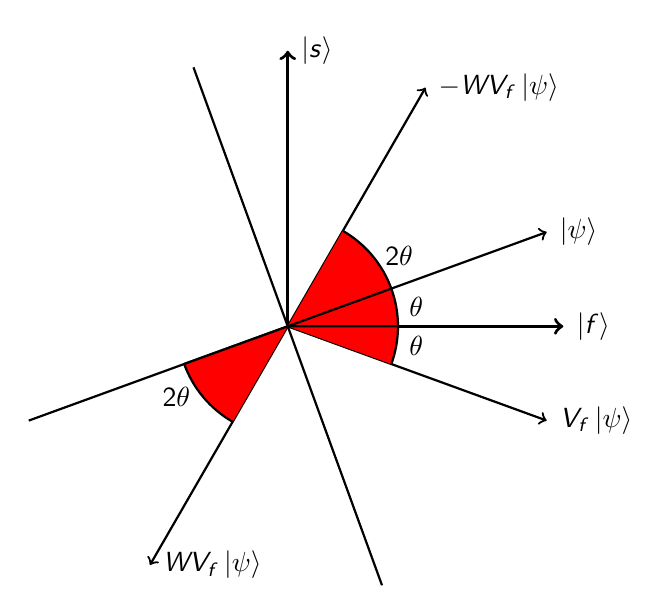
\begin{tikzpicture}[scale=0.7]
\draw[very thick,->] (0,0) -- (5,0) node[right=1pt] {$\ket{f}$};
\draw[very thick,->] (0,0) -- (0,5) node[right=1pt] {$\ket{s}$};
\draw[thick,->] (0:0) -- (20:5) node[right=1pt] {$\ket{\psi}$};
\filldraw[thick,fill=red] (0,0) -- (2,0) arc[start angle=0, end angle=20, radius=2] node[pos=0.5,right=1pt] {$\theta$};
\draw[thick,->] (0:0) -- (-20:5) node[right=1pt] {$V_f\ket{\psi}$};
\filldraw[thick,fill=red] (0,0) -- (2,0) arc[start angle=0, end angle=-20, radius=2] node[pos=0.5,right=1pt] {$\theta$};
\draw[thick] (0:0) -- (110:5);
\draw[thick] (0:0) -- (-70:5);
\draw[thick] (0:0) -- (200:5);
\draw[thick,->] (0:0) -- (240:5) node[right=1pt] {$WV_f\ket{\psi}$};
\filldraw[thick,fill=red] (0,0) -- (200:2) arc[start angle=200, end angle=240, radius=2] node[pos=0.5,left=1pt] {$2\theta$};
\draw[thick,->] (0:0) -- (60:5) node[right=1pt] {$-WV_f\ket{\psi}$};
\filldraw[thick,fill=red] (0,0) -- (20:2) arc[start angle=20, end angle=60, radius=2] node[pos=0.5,right=1pt] {$2\theta$};
\end{tikzpicture}
}
\end{frame}
\begin{frame}{Analysis of Grover's algorithm}
\begin{equation*}
(-WV_f)^k \ket{+} = \sin((2k + 1)\theta)\ket{s} + \cos((2k+1)\theta)\ket{f}
\end{equation*}
The probability of success is \emm{$\sin^2((2k+1)\theta)$}.

\vspace{1em}
Choose $k$ satisfying
\begin{equation*}
(2k+1)\theta \approx \frac{\pi}2
\iff k \approx \frac{\pi}{4\theta}
\end{equation*}
Here, $\sin\theta = \sqrt{\frac{M}{N}} \iff \theta\approx\sqrt{\frac{M}{N}}$.
Hence, $k\approx \frac{\pi}4\sqrt{\frac{N}{M}}$.

\vspace{2em}
[Grover 1996]
\end{frame}

\begin{frame}{Grover's algorithm}
[Boyer, Brassard, H\o yer, and Tapp 1998]
\begin{enumerate}
\item Initialize $m = 1$ and set $\lambda = 8/7$.
\item Choose an integer $j$ uniformly from $0,1,\dotsc, m$.
\item Apply Grover's algorithm with $j$ iterations.
\item If solution is not found, set $m\leftarrow\min(\lambda m, \sqrt{N})$ and go back to setp 2.
\end{enumerate}

\vspace{3em}
\centering
This algorithm solves the ``OR problem''\\
 with $O(\sqrt{N/M})$ query for $U_f$.
\end{frame}

\begin{frame}{Applications of Grover's algorithm}
\begin{itemize}
\setlength{\itemsep}{2em}
\item $O^*(2^{n/2})$ algorithm for SAT.
\item $O^*(2^{n/3})$ algorithm for the subset sum [Brassard et al.\ 1997].
\item $O(1.728^{n})$ algorithm for the travelling salesman problem\\
{[Ambainis et al.\ 2019]}.
\item $O(1.914^{n})$ algorithm for the graph coloring problem\\
{[Shimizu and Mori 2019]}.
\end{itemize}
\end{frame}

\begin{frame}{Optimality of Grover's search}
\begin{align*}
\ket{\psi_x^i} &:= (U_k V_x U_{k-1} V_x\dotsm  U_{i+1} V_x) (U_iU_{i-1} \dotsm U_1) \ket{\psi_0}\\
\ket{\psi_x^0} &= U_k V_x U_{k-1} V_x \dotsm V_x U_1 V_x\ket{\psi_0}\\
\ket{\psi_x^{k}} &= U_k U_{k-1} \dotsm U_1 \ket{\psi_0}\\
\end{align*}
For any ``\emm{distance}'' function $D$ for $\left\{\ket{a}\in\mathbb{C}^N\mid \braket{a|a} = 1\right\}$,
\begin{align*}
& \frac1N \sum_x D\left(\ket{x},\ket{\ne x}\right)\\
%&= \frac1N \sum_x\left\|\ket{x}-\ket{\psi_x^0}+\sum_{i=0}^{k-1} \left(\ket{\psi_x^i} - \ket{\psi_x^{i+1}}\right) + \ket{\psi_x^k} - \ket{\ne x}\right\|\\
&\le \frac1N \sum_x\left(D\left(\ket{x}, \ket{\psi_x^0}\right)+\sum_{i=0}^{k-1} D\left(\ket{\psi_x^i}, \ket{\psi_x^{i+1}}\right) + D\left(\ket{\psi_x^k}, \ket{\ne x}\right)\right).
\end{align*}
\end{frame}

\begin{frame}{``Distance'' function}
%\begin{align*}
%&\frac1N \sum_x\left(D\left(\ket{x}, \ket{\psi_x^0}\right)+\sum_{i=0}^{k-1} D\left(\ket{\psi_x^i}, \ket{\psi_x^{i+1}}\right) + D\left(\ket{\psi_x^k}, \ket{\ne x}\right)\right).
%\end{align*}
Let
\begin{align*}
D(\ket{a}, \ket{b}):= \emm{\arccos \left|\braket{a|b}\right|}.
\end{align*}
For any normalized $\ket{a},\,\ket{b},\,\ket{c}$,
\begin{align*}
\begin{bmatrix}
1&\braket{a|b}&\braket{a|c}\\
\braket{b|a}&1&\braket{b|c}\\
\braket{c|a}&\braket{c|b}&1
\end{bmatrix}
\succeq 0.
\end{align*}
The determinant of this matrix is
\begin{align*}
&1 + \braket{a|b}\braket{b|c}\braket{c|a} + \braket{a|c}\braket{b|a}\braket{c|b}\\
&- \braket{b|c}\braket{c|b} - \braket{a|c}\braket{c|a} - \braket{a|b}\braket{b|a}\ge 0.
\end{align*}
\end{frame}

\begin{frame}{The triangle inequality}
\begin{align*}
&1 + \braket{a|b}\braket{b|c}\braket{c|a} + \braket{a|c}\braket{b|a}\braket{c|b}\\
&- |\braket{b|c}|^2 - |\braket{a|c}|^2 - |\braket{a|b}|^2\ge 0\\
\Longrightarrow\quad& 1 + |\braket{a|b}\braket{b|c}\braket{c|a}| + |\braket{a|c}\braket{b|a}\braket{c|b}|\\
&- |\braket{b|c}|^2 - |\braket{a|c}|^2 - |\braket{a|b}|^2\ge 0\\
\Longleftrightarrow\quad& 1 + \cos(\theta_{ab})\cos(\theta_{bc})z + z\cos(\theta_{ab})\cos(\theta_{bc})\\
&- \cos^2(\theta_{bc}) - z^2 - \cos^2(\theta_{ab}) \ge 0\\
\Longleftrightarrow\quad& 
z^2 - 2\cos(\theta_{ab})\cos(\theta_{bc}) z\\
&+ \cos^2(\theta_{bc}) + \cos^2(\theta_{ab}) -1 \le 0\\
\Longleftrightarrow\quad& 
\left(z - \cos(\theta_{ab})\cos(\theta_{bc})\right)^2- \cos^2(\theta_{ab})\cos^2(\theta_{bc})\\
&+ \cos^2(\theta_{bc}) + \cos^2(\theta_{ab}) -1 \le 0\\
\Longleftrightarrow\quad& 
\left(z - \cos(\theta_{ab})\cos(\theta_{bc})\right)^2 \le \left(1-\cos^2(\theta_{ab})\right)\left(1-\cos^2(\theta_{bc})\right)
\end{align*}
\end{frame}

\begin{frame}{The triangle inequality}
\begin{align*}
&\left(z - \cos(\theta_{ab})\cos(\theta_{bc})\right)^2 \le \sin^2(\theta_{ab})\sin^2(\theta_{bc})\\
\Longrightarrow\quad& z \ge \cos(\theta_{ab})\cos(\theta_{bc}) - \sin(\theta_{ab})\sin(\theta_{bc})\\
\Longleftrightarrow\quad& z \ge \cos(\theta_{ab}+\theta_{bc})\\
\Longleftrightarrow\quad& \arccos(|\braket{c|a}|) \le \theta_{ab}+\theta_{bc}\qquad \text{$\arccos$ is decreasing for $[-1,+1]$}\\
\Longleftrightarrow\quad& \emm{\theta_{ca} \le \theta_{ab}+\theta_{bc}}
\end{align*}
\end{frame}

\begin{frame}{Inequalities}
\small
For the simplicity, we assume $\ket{\psi_0}=\frac1{\sqrt{N}}\sum_x\ket{x}$ and $\{U_i\}_{i=1,\dotsc,k}$ are symmetric, i.e., $PU_iP^\dagger = U_i$ for any permutation matrix $P$.
\begin{align*}
&  \emm{\frac{\pi}2} = \frac1N \sum_x D\left(\ket{x},\ket{\ne x}\right)\\
%&= \frac1N \sum_x\left\|\ket{x}-\ket{\psi_x^0}+\sum_{i=0}^{k-1} \left(\ket{\psi_x^i} - \ket{\psi_x^{i+1}}\right) + \ket{\psi_x^k} - \ket{\ne x}\right\|\\
&\le \frac1N \sum_x\left(D\left(\ket{x}, \ket{\psi_x^0}\right)+\sum_{i=0}^{k-1} D\left(\ket{\psi_x^i}, \ket{\psi_x^{i+1}}\right) + D\left(\ket{\psi_x^k}, \ket{\ne x}\right)\right).
\end{align*}
\begin{align*}
%D\left(\ket{x},\ket{\ne x}\right) &= \frac{\pi}2\\
\frac1N\sum_x D\left(\ket{x},\ket{\psi_x^0}\right) &= \frac1N\sum_x \arccos\left(|\braket{x|\psi_x^0}|\right)\\
\le \arccos\left(\frac1N\sum_x |\braket{x|\psi_x^0}|\right)
&\emm{=} \arccos\left(\sqrt{p_{\mathsf{succ}}}\right).\\
\frac1N\sum_x D\left(\ket{\psi_x^k},\ket{\ne x}\right) &= \frac1N\sum_x \arccos\left(|\braket{\psi_x^k|\ne x}|\right)\\
\le \arccos\left(\frac1N\sum_x |\braket{\psi_x^k|\ne x}|\right)
&\emm{=} \arccos\left(\sqrt{1-\frac1N}\right).
\end{align*}
\end{frame}

\begin{frame}{Inequalities}
\begin{align*}
\frac1N\sum_x D\left(\ket{\psi_x^i},\ket{\psi_x^{i+1}}\right) &= \frac1N\sum_x \arccos\left(|\braket{\psi_x^i|\psi_x^{i+1}}|\right)\\
= \frac1N\sum_x \arccos\left(|\bra{\varphi}V_x\ket{\varphi}|\right)
&\le \arccos\left(\frac1N\sum_x |\bra{\varphi}V_x\ket{\varphi}|\right)\\
\le \arccos\left(\left|\frac1N\sum_x \bra{\varphi}V_x\ket{\varphi}\right|\right)
&= \arccos\left(\left|\bra{\varphi}\left(\emm{1-\frac2N}\right)I\ket{\varphi}\right|\right)\\
&= \arccos\left(\emm{1-\frac2N}\right)\\
\end{align*}
\end{frame}

\begin{frame}{Put everything together}
\begin{align*}
&  \frac{\pi}2 = \frac1N \sum_x D\left(\ket{x},\ket{\ne x}\right)\\
%&= \frac1N \sum_x\left\|\ket{x}-\ket{\psi_x^0}+\sum_{i=0}^{k-1} \left(\ket{\psi_x^i} - \ket{\psi_x^{i+1}}\right) + \ket{\psi_x^k} - \ket{\ne x}\right\|\\
&\le \frac1N \sum_x\left(D\left(\ket{x}, \ket{\psi_x^0}\right)+\sum_{i=0}^{k-1} D\left(\ket{\psi_x^i}, \ket{\psi_x^{i+1}}\right) + D\left(\ket{\psi_x^k}, \ket{\ne x}\right)\right)\\
&\le \arccos\left(\sqrt{p_{\mathsf{succ}}}\right)+k\arccos\left(1-\frac2N\right)+ \arccos\left(\sqrt{1-\frac1N}\right)
\end{align*}
Since \emm{$\theta = \arccos\left(\sqrt{\frac{N-1}{N}}\right)$},
\begin{align*}
&\frac{\pi}2\le \arccos\left(\sqrt{p_{\mathsf{succ}}}\right)+2k\theta+ \theta\\
\iff &\cos\left(\frac{\pi}2-(2k+1)\theta\right)\ge \sqrt{p_{\mathsf{succ}}}\qquad \text{if $(2k+1)\theta\le \frac{\pi}2$}\\
\iff &\sin^2\left((2k+1)\theta\right)\ge p_{\mathsf{succ}}.
\end{align*}
[Zalka 1999]
\end{frame}

\begin{frame}{Summary}
\begin{itemize}
\setlength{\itemsep}{2em}
\item Grover's search solves the quantum searching problem in time $O(\emm{\sqrt{N}})$.
\item Grover's search is exactly \emm{optimal} if $M=1$.
\item For general $M$, Grover's search is \emm{asymptotically optimal}.
\end{itemize}
\end{frame}

\end{document}
